\section{Transformationssprache ODHQL}
In diesem Kapitel wird die Transformationssprache ODHQL erläutert.
\subsection{Syntax}

Die Syntax von \acs{odhql} orientiert sich stark an SELECT aus \acs{ansi} \acs{sql}.

Eine formale Beschreibung der Transformationssprache ist in \cref{app:odhql-syntax} zu finden.

\subsection{Unterstützte Features}

\cref{tab:pd:transformation-lang-impl} beschreibt die unterstützten Features:
\mytable{lX}{
  \textbf{Anforderung} & \textbf{Beschreibung}\\
  \midrule
  \textbf{Mapping} & Felder können mit oder ohne Alias angegeben werden. Falls kein Alias vorhanden ist wird der Feldname beibehalten. Es ist möglich, Sonder- und Leerzeichen zu verwenden, indem der Feldname in doppelten Anführungszeichen geschrieben wird. \\
  \textbf{Default-Werte} & Unterstützt werden Integer, Float, sowie Strings (in einfachen Anführungszeichen). \\
  \textbf{Joins} & Es muss immer mindestens eine Datenquelle angegeben werden. Falls mehr verwendet werden sollen muss mindestens eine Join-Bedingung vorhanden sein (es werden mehrere Join-Bedingungen unterstützt, jedoch nur per ``and''-Verknüpfung). Neben Inner Joins werden auch Left, Right und Full Outer Joins unterstützt. \\
  \textbf{Filter/Prädikate} & Vorhandene Filter beinhalten: ``is null'', ``in (...)'', relationale Operatoren wie ``='', ``<'', etc., Prädikate und ``like `regex'\ '' (letzteres ist eine Abweichung von ANSI SQL, welches eine separate Syntax für Like-Filter hat) \\
  \textbf{Erweiterbare Funktionen} & Alle Funktionen werden über eine Function Registry in Python aufgerufen und können daher einfach erweitert werden. \\
  \textbf{Sortierung} & Es kann eine Order By-Klausel angegeben werden. Falls Unions verwendet werden muss die Order By-Klausel am Ende angegeben werden, nicht pro Query. \\
  \textbf{Unions} & Mehrere Queries können per Union zusammengefügt werden. Die Implementation entspricht dem UNION ALL aus SQL, es findet also keine Deduplizierung statt. \\
}{Durch \acs{odhql} implementierte Features}{pd:transformation-lang-impl}

Jede Transformation definiert eine Liste von Feldern oder Werten, sowie mindestens eine Datenquelle. 

\subsection{Beispiele}
Folgende Items sind in der Feld-Liste erlaubt:
\begin{description}
\item[Feld] Name des Feldes, mit dem Namen oder Alias der Datenquelle als Präfix. Feldnamen und Aliase können in doppelten Anführungszeichen geschrieben werden, z.B. wenn Sonder- oder Leerzeichen verwendet werden sollen. Zu beachten ist, dass Feldnamen immer einen Präfix brauchen, auch ausserhalb der Feld-Liste.
\begin{src}{sql}
a.beschreibung, a.geom as geometry, a."Zentroid X [m]"
\end{src}
\item[Wert] Integer, Float, Boolean, Null oder String in einfachen Anführungszeichen. Es muss zwingend ein Alias angegeben werden. 
\begin{src}{sql}
1 as one, 3.14 as pi, false as active, 'sun' as local_star
\end{src}
\item[Funktion] Ein Funktionsaufruf besteht aus einem Namen sowie einer Liste von Argumenten in runden Klammern. Funktionsaufrufe können verschachtelt werden.
\begin{src}{sql}
 cast(a.pi, 'float') as pi,
 concat('POINT(', cast(v0.x, 'string'), ' ', cast(v0.y, 'string'), ')')) as geometry
\end{src}
\end{description}

Datenquellen können per Join verknüpft werden.
\begin{src}{sql}
  from "Gebäude" as geb join Strassen as str on geb.str_id = str.id
\end{src}

Unterstützt werden Inner Join, Left, Right und Full Outer Join. Dabei wird jeweils die einfachste Syntax\footnote{\texttt{join}, \texttt{left join}, \texttt{right join} und \texttt{full join}.} verwendet.

Als Filter können folgende Ausdrücke verwendet werden:
\begin{description}
\item[Relationale Operatoren] Unterstützt werden die Operatoren `=', `!=', `<', `>', `<=', `>='.
\begin{src}{sql}
a.nr > 4, a.active = false
\end{src}
\item[Like] Anders als bei SQL verwendet der Like-Operator von \acs{odhql} implementationsbedingt Reguläre Ausdrücke (Python Syntax\footnote{Siehe \url{https://docs.python.org/2/library/re.html\#regular-expression-syntax}}).
\begin{src}{sql}
a.beschreibung like 'Z[uü]rich', a.beschreibung not like 'Z[uü]rich'
\end{src}
\item[In] Sucht den Ausdruck in einer Liste von Elementen.
\begin{src}{sql}
a.nr in (3, 4, 5), a.nr not in (2, 6, 7)
\end{src}
\item[Null-Check] Prüft, ob ein Ausdruck Null (bzw. None) ist.
\begin{src}{sql}
a.optional_field is null, a.mandatory_field is not null
\end{src}
\end{description}

Die Resultate mehrerer Queries werden mit Union zusammengehängt. Dies verhält sich wie ``union all'' in SQL, d.h. es findet keine Deduplizierung der Daten statt.
\begin{src}{sql}
  select a.description, a.geometry from A as a
   union
  select b.description, b.geometry from B as b
\end{src}
Zu beachten ist, dass die Feld-Listen der Queries kompatibel sein müssen.
\newline

\subsection{Abstrakter Syntax-Baum (AST)}
Der ODHQL-Parser analysiert die Abfrage in Text-Form und wandelt diese in einen Abstrakten Syntax Baum (AST) um. Dieser wird anschliessend vom Interpreter verwendet, um die Transformation auf die Daten anzuwenden.

\cref{fig:pd:odhql-ast-toplevel} zeigt die Toplevel-Struktur des Abstrakten Syntax-Baums.
\begin{figure}[H]
\centering
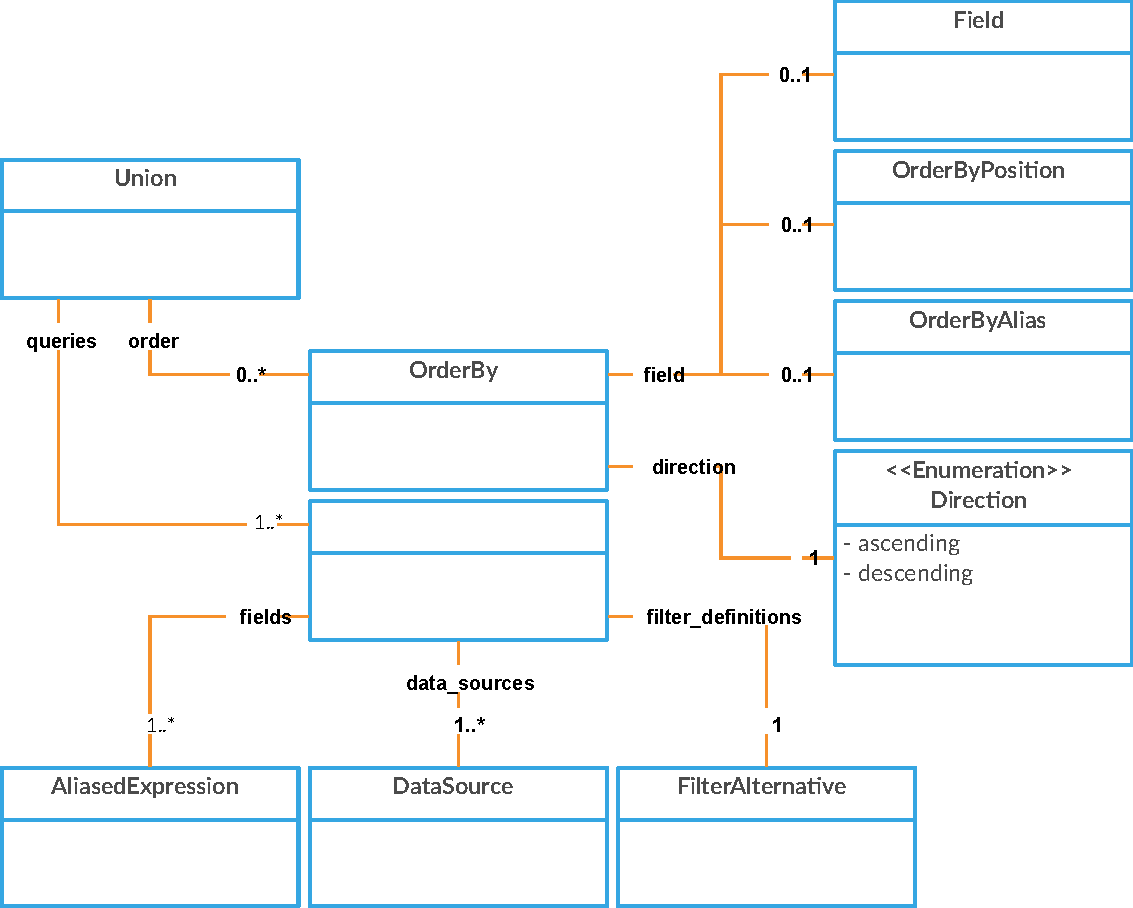
\includegraphics[width=0.8\linewidth]{fig/odhql-ast-union.pdf}
\caption{AST: Unions}
\label{fig:pd:odhql-ast-toplevel}
\end{figure}

Die in \cref{fig:pd:odhql-ast-expressions} beschriebenen Ausdrücke repräsentieren Felder, Werte, Funktionsaufrufe, etc.
\begin{figure}[H]
\centering
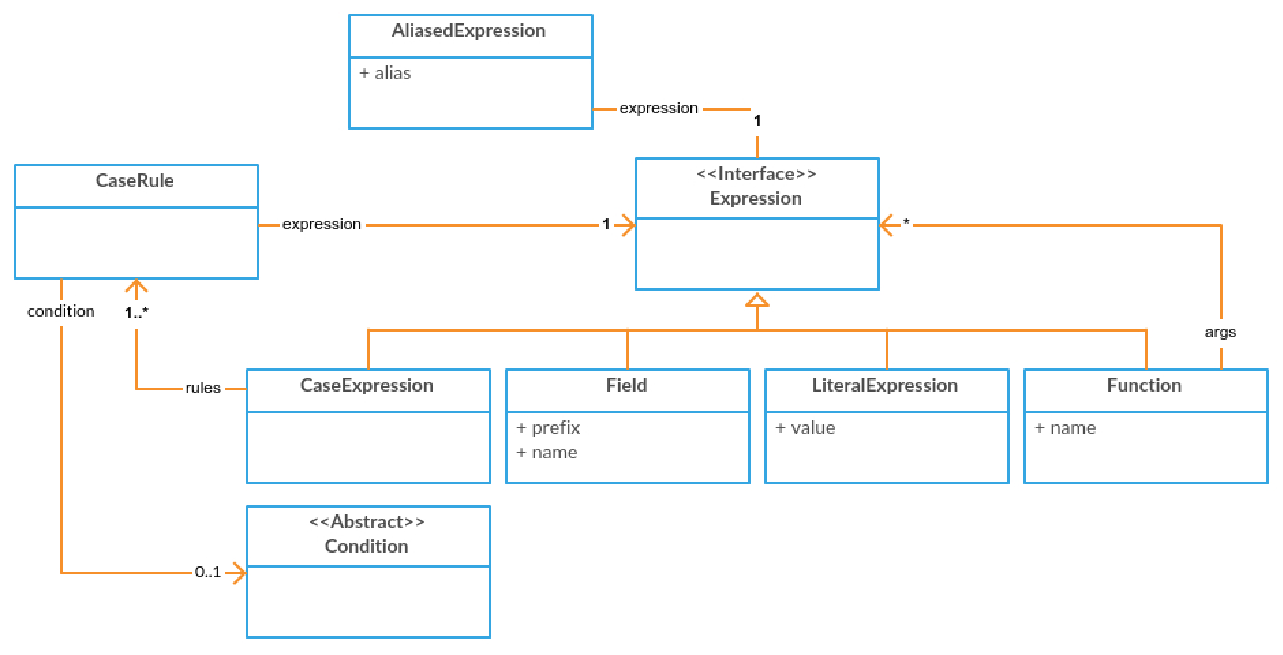
\includegraphics[width=0.8\linewidth]{fig/odhql-ast-expression.pdf}
\caption{AST: Ausdrücke}
\label{fig:pd:odhql-ast-expressions}
\end{figure}

\cref{fig:pd:odhql-ast-datasources} zeigt auf, wie Datenquellen repräsentiert werden.
\begin{figure}[H]
\centering
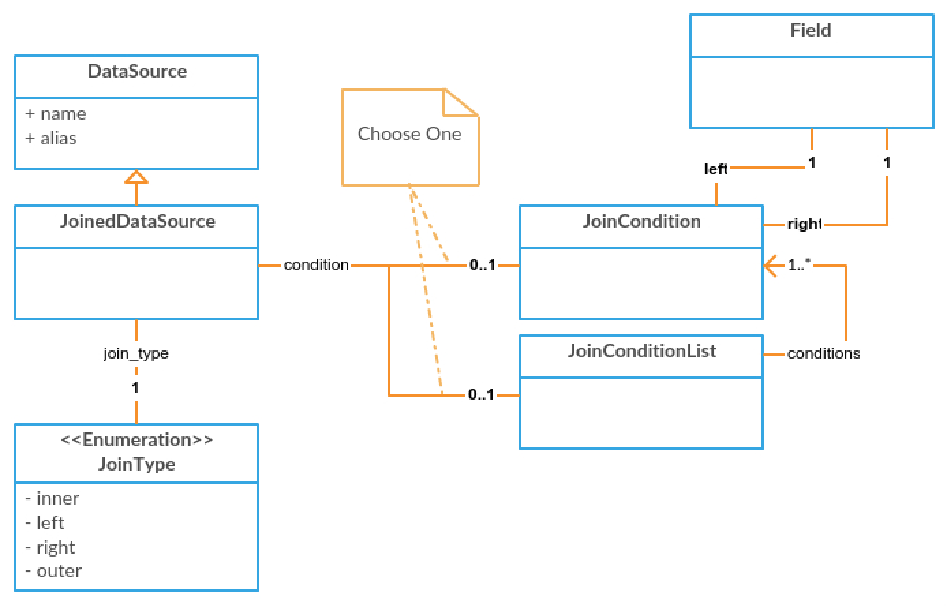
\includegraphics[width=0.8\linewidth]{fig/odhql-ast-datasources.pdf}
\caption{AST: Datenquellen}
\label{fig:pd:odhql-ast-datasources}
\end{figure}

Filter werden wie in \cref{fig:pd:odhql-ast-filter} beschrieben dargestellt.
\begin{figure}[H]
\centering
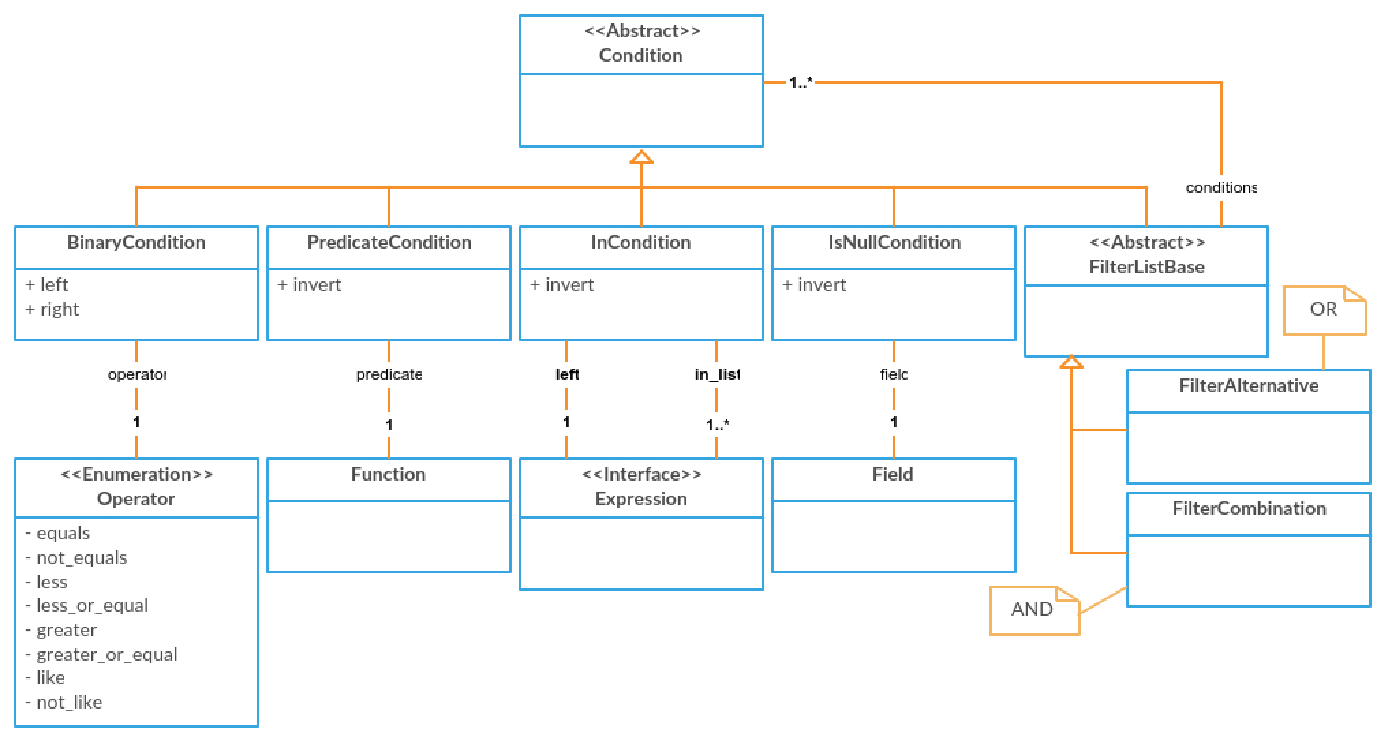
\includegraphics[width=0.8\linewidth]{fig/odhql-ast-filter.pdf}
\caption{AST: Filter}
\label{fig:pd:odhql-ast-filter}
\end{figure}

\subsection{Interpreter}
Mit Pandas und NumPy ist bereits eine API für viele SQL-ähnliche Operationen wie Selektion, Joins und diverse String- und Geometriefunktionen (GeoPandas Erweiterung) vorhanden. Die Herausforderung bei der Entwicklung des Interpreters liegt somit einerseits in einer performanten und möglichst fehlerfreien Ausführung, andererseits der Erweiterbarkeit durch eigene Funktionen.

\begin{figure}[H]
\centering
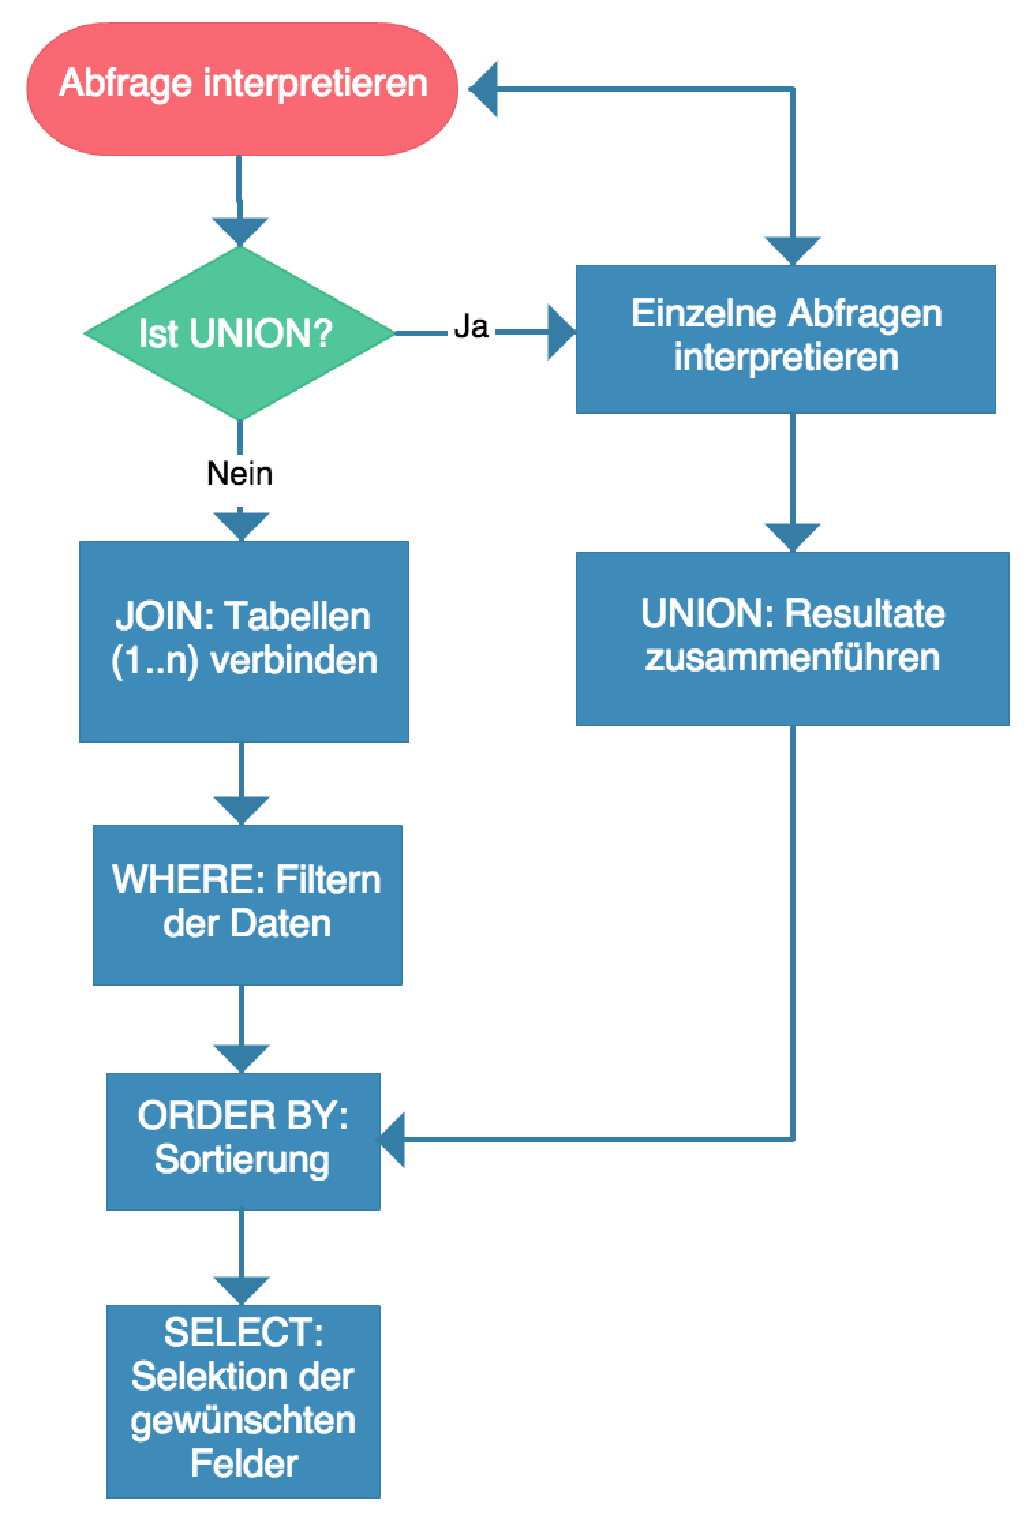
\includegraphics[width=0.6\linewidth]{fig/odhql-flow.pdf}
\caption{High-level Ablauf der Abfrage-Interpretation}
\label{fig:pd:odhql-flow}
\end{figure}


\subsection{Funktionen}
Die Funktionen der \acs{odhql} wurden möglichst erweiterbar implementiert. Neue Funktionen erben von der Klasse \path{VectorizedFunction} und implementieren die Methode \path{apply}. 

Durch die Vererbung und der zugrunde liegenden Python-Metaklasse wird die neue Funktion automatisch registriert und ist sofort mit dem Klassennamen verfügbar. Der Name kann durch das statische Attribut \path{name} auch explizit gesetzt werden. Die Anzahl der Funktionsparameter werden vom Interpreter bzw. von der Execution Engine der Funktionen via Reflection sichergestellt. Für die Überprüfung der Argumente ist jede Funktion selbst zuständig. Die Parent-Klasse bietet jedoch bereits einige Assertion-Methoden z.B. für Datentypen, Listen und Geometrien.

Ein Beispiel einer solchen Funktion ist in \cref{src:pd:odhql-function} ersichtlich. Hierbei wird nach der Überprüfung der Argumente direkt an die Pandas-Methode \path{str.pad} weiterdelegiert.

\begin{srclst}[label=src:pd:odhql-function]{python}{Beispiel-Implementation der ODHQL-Funktion \texttt{PAD()}}
from hub.odhql.functions.core import VectorizedFunction

class Pad(VectorizedFunction):
    name = 'PAD'

    def apply(self, strings, width, side):
        self.assert_str('string', strings)
        self.assert_in('side', side, ['left', 'right', 'both'])
        self.assert_int('width', width)
        return strings.str.pad(width, side)
\end{srclst}